\begin{refsection}
\chapter{Replication: Surviving Andersonville}
\label{andersonville}
\textbf{Aksel Erbahar, Cecilia Heuser, Victor K\"ummritz, Bastiaan Quast}

\section*{Abstract}
We replicate \textcite{costa2007surviving}. We are able to replicate all the result from the paper. The authors make a number of choices in order to arrive to the results published. We raise some concerns regarding some of these choices. For example, the authors treat the POWs of the two Andersonville camps as if they were in the same camp. This inflates size of the POWs social network, which is used as the explanatory variable. When we make choices which to us seem more defendable, we cannot, quantitatively and qualitatively, replicate the authors' results.

\section{Summary of the paper}
\textcite{costa2007surviving} try to estimate the effect of quality and size of social networks on ensuring the survival of prisoners of war (POW) in POW camps. To examine the relationship the authors combine two datasets, a longitudinal dataset of Union Army soldiers and a cross-sectional dataset of the POW camp in Andersonville. 

The empirical specification for the longitudinal data that measures the effect of the size of the network is as follows:

\begin{equation} \label{eq:ht}
h(t) = \exp ( \beta_1 F + \beta_2 I + \beta_3 M )
\end{equation}

where $h$ is hazard at time $t$, $F$ is the number of friends (=social network), $I$ are individual characteristics and $M$ macro camp conditions. The number of friends is measured as the number of POWs of the same company and varies by month due to deaths or camp transfers. As it might capture the lagged mortality of the group, the authors use as second strategy the initial number of friends as a time-invariant proxy. In addition, they instrument for the number of friends using the number of net camp transfers combined with a dummy indicating whether the POW was transferred to account for omitted variables. 
The specification for the Andersonville data in turn is a probit model:

\begin{align}
Pr(S = 1) &= \Phi (\beta_1 F + \beta_2 F) \label{s1} \\
Pr(S = 1) &= \Phi (\beta_1 F_i + \beta_2 F_{ij} + \beta_3 I | ethnicity = j) \label{s1b} 
\end{align}

where equation \autoref{s1} examines quantity and \autoref{s1b} quality of the social network. The measure for number of friends here is the number of POWs from the same company in Andersonville.

The longitudinal data indicates that POWs had special characteristics. For instance, they were likely to be volunteers, and from companies with more wounded or dead. POWs with more friends were typically US-born and wealthier while Irish and older men had less friends. Concerning survival rates, Kaplan-Meier hazard rates show that POWs captured later (after 1963 when the Union and the Confederate Army stopped exchanging POWs) have lower survival rates. They also show that survival rates were higher for POWs with 10 or more friends. In addition, the rates show that it takes 50 days until there is a divergence in survival between POWs with and without friends. The exponential function estimates that an additional friend leads to a 0.98 times lower mortality hazard. An increase in the number of friends from 0 to 5 (5 to 10), decreases the predicted probability of death from 0.31 to 0.28 (0.26) while a spline specification provides evidence that the effect is greatest for the first two friends. In addition, survival is more likely for POWs that had survived at least one or two months. Factors increasing mortality are the number of men in the camp, low rank, high age, and height among others. Insignificant variables are for instance wealth and marital status. There is no evidence for individual heterogeneity. The use of a Weibull specification indicates no duration dependence (toughen up effects). Interestingly though, a Cox model gives no significant effect of friends which the authors interpret as a result of their loss of power due to the small sample size. Robustness checks, including the IV approach and the effect of friends transferred in, confirms the significant effect of friends. Finally, the cross-sectional results provide evidence that having the same last name, being from the same town for smaller towns, ethnic similarity and having a sergeant or a higher rank in one's network are all important factors in raising survival probabilities which in turn shows that the quality of social networks matters.

In summary, Costa and Kahn are able to show that quantity and quality of social networks mattered for survival in civil war POW camps. Potential explanations for this are the sharing of scarce resources, moral support and protection from other prisoners.

\section{Data}
The raw data for the first part of the paper is extracted from the Union Army dataset readily accessible at \url{http://www.cpe.uchicago.edu}. This dataset draws information from censuses, medical records and military pension records linking military, socioeconomic and health information for nearly $40,000$ white males that served in the Union Army during the Civil War. For the second part, the Andersonville database is available at \url{http://www.itd.nps.gov/cwss} but only as a ``searchable version'', which allows viewing the information for one soldier at a time, and more convenient formats are not readily available.

The datasets provided for the estimations alongside with the publication are already partially processed parts of the raw data available online. No clear guidance is given as to what steps were taken to go from the raw data to the files provided, and matching both things proved to be less than straightforward. In view of this, we decided to proceed with the replication using the files provided by the authors, pointing out along the way the cases where potential problems in them seemed likely given the raw data we observed. Taking those files as starting points, it is possible to reproduce the tables and graphs published in the paper, so in this sense we can say that the data set is complete. Originally, some of the data required by the published .do files was not included in the published data files, but the authors provided it promptly upon our request and added it subsequently to the online files of the publishing journal.

The data and .do files provided do not describe or label many of the variables used, nor does the limited variable description in the Appendix cover all of them. A very thorough description of the variables in the raw data set can be found at its online source, but the match between this and the variables in the files provided is not straightforward or complete, since some of them are already created by the authors from the raw data. The description of the data itself, mainly of the variables that are used most often, is succinct but adequate, with Table 1 and Table 2 presenting some relevant descriptive traits. Despite this, some attention should be drawn to the fact that some of the variables have a relevant share of missing values (only the highest number of observations is reported), a point that will be commented in detail later on.

\section{Stata code and interpretation}
All codes run to their full extent, and produce the estimations presented in the paper, with minor differences that we describe in detail below. The codes themselves are not commented at all and include plenty of estimations and specifications not included in the published paper, as well as unexplained data processing steps. No exporting commands were set up, or log files kept, which might be the root of some of the rounding and significance discrepancies we have found. 

In what follows, all reproduced tables are presented with a comment on the differences found (in bold), whenever there were any.

\subsection{Tables}
Table 1: This table presents the means of most variables later used for estimation, dividing observations in POWs and NON POWs, to illustrate ex ante differences in observables between them.

\begin{table}[bt]
\centering
\caption{Characteristics of Soldiers by POW Status}
\label{characteristics}
\begin{tabular}{lllllll}
\hline
                           & All   & Obs.  & Never POW & Obs.  & POW   & Obs. \\
US born                    & 0.745 & 35007 & 0.745     & 31967 & 0.743 & 3040 \\
US born corrected          & 0.747 & 34941 & 0.745     & 31966 & 0.759 & 2975 \\
Irish                      & 0.087 & 34941 & 0.086     & 31966 & 0.102 & 2975 \\
German                     & 0.074 & 34941 & 0.075     & 31966 & 0.062 & 2975 \\
British                    & 0.039 & 34941 & 0.039     & 31966 & 0.033 & 2975 \\
Other                      & 0.054 & 34941 & 0.055     & 31966 & 0.043 & 2975 \\
Artisan                    & 0.2   & 34941 & 0.199     & 31966 & 0.211 & 2975 \\
Farmer corrected           & 0.505 & 34941 & 0.505     & 31966 & 0.508 & 2975 \\
Professional or proprietor & 0.075 & 34941 & 0.077     & 31966 & 0.061 & 2975 \\
Laborer                    & 0.212 & 34941 & 0.212     & 31966 & 0.212 & 2975 \\
Unknown                    & 0.007 & 34941 & 0.007     & 31966 & 0.008 & 2975 \\
Enlisted in 1861           & 0.21  & 35007 & 0.205     & 31967 & 0.263 & 3040 \\
Enlisted in 1861 corrected & 0.21  & 34878 & 0.205     & 31906 & 0.269 & 2972 \\
Enlisted in 1862                  & 0.344   & 34878 & 0.331   & 31906 & 0.487  & 2972 \\
Enlisted in 1863                  & 0.068   & 34878 & 0.066   & 31906 & 0.087  & 2972 \\
Enlisted in 1864                  & 0.256   & 34878 & 0.266   & 31906 & 0.147  & 2972 \\
Enlisted in 1865                  & 0.122   & 34878 & 0.132   & 31906 & 0.009  & 2972 \\
Volunteer                         & 0.909   & 34941 & 0.905   & 31966 & 0.951  & 2975 \\
Height in inches                  & 67.599  & 34941 & 67.589  & 31966 & 67.709 & 2975 \\
Household property income in 1860 & 534.155 & 13769 & 531.734 & 12509 & 558.2  & 1260 \\
Company birthplace fragmentation  & 0.642   & 34941 & 0.644   & 31966 & 0.62   & 2975 \\
Company occupation fragmentation  & 0.559   & 34941 & 0.558   & 31966 & 0.57   & 2975 \\
Fraction company died as non-POWs & 0.135   & 34941 & 0.131   & 31966 & 0.182  & 2975 \\
\end{tabular}
\end{table}

We have added to \autoref{characteristics} the number of observations per variable, not originally included in the paper, in order to highlight the fact that some of them have significant amounts of missing values, something that should be kept in mind later at the estimation stage. In this table, the case in point is Household property income in 1860, which is used in most of the specifications proposed, but as will be discussed for later tables, this is a pattern common to all the variables imported from census data. 
Additionally, considering the number of observations for each of the variables leads to the suggestion of a small correction for three of the dummy variables describing categories: US born, farmer and enlisted in 1861. The initial data file is missing these variables, which are likely to have been dropped as the basis category for estimation purposes in some other use of the data. They were then rebuilt in the .do file from the remaining categories in such a way that generated zeroes for some observations that should have been missing (except for farmer, which is not included at all in the file). For example: as provided by the code, US born has $35,007$ observations, whereas other nationality dummies, all built from the same original variable, have $34,941$. The correction proposed then, is to set these dummies to missing whenever the other categories of their class are missing, which slightly changes their descriptive statistics (for example the mean of US born goes from $0.745$ to $0.747$ when this correction is implemented).

Remaining discrepancies are minor and could be due to some kind of rounding difference. An alternative explanation for these differences is that the table was produced from a slightly different dataset. Considering that even the most populous variables present over 500 observations less than the amount declared in the paper, and the fact that one of the variables (farmer) is not included in the data file at all, we consider the second option to be more likely, which would also explain the minor differences in the means of Artisan, British, Height in inches, etc.

A last and minor comment is that the inclusion of the variable volunteer is surprising, since by sample design the Union Army dataset was restricted to white volunteer infantry regiments. The inclusion of this variable when comparing POWs and non POWs probably responds to the point raised in the paper about POWs not being representative of all soldiers, for example in ideology (p.1471). A variable that reflects that both POWs and non POWs volunteered in similar proportions would suggest homogeneity between POWs and non POWs in this dimension and, hence, increase  external validity. The similarities observed in Table 1 between POWs and non POWs in their mean of volunteer do not reflect that, since they are both close to one by construction. Any individuals not listed as volunteers, either correspond to the very few drafted men, or are actually soldiers that re-enlisted as commissioned officers, but were originally volunteers, as explained in the codebooks for the source data.

\ref{friends}: This table describes the variables later used in the main regressions, focusing in this case only on POWs.  It also presents separately their mean and standard errors for the subsamples of POWs with few (less than 3) and many friends (three or more). 

\begin{sidewaystable}
\caption{Characteristics of POWs by Number of Friends in First Two Weeks of Captivity}
\label{friends}
\begin{tabular}{llllllllll}

                                  & \multicolumn{3}{l}{All} & \multicolumn{3}{l}{Few friends ($<3$)} & \multicolumn{3}{l}{Many friends ($>=3$)} \\
                                  & Mean                    & Std. err.                            & No. obs.                               & Mean & Std. err. & No. obs. & Mean & Std. err. & No. obs. \\
US born                           & 0.731                   & 0.444                                & 1976                                   & 0.708 & 0.455 & 990 & 0.754 & 0.431 & 986 \\
Irish                             & 0.12                    & 0.325                                & 1976                                   & 0.115 & 0.319 & 990 & 0.125 & 0.331 & 986 \\
German                            & 0.063                   & 0.243                                & 1976                                   & 0.081 & 0.273 & 990 & 0.045 & 0.207 & 986 \\
British                           & 0.034                   & 0.182                                & 1976                                   & 0.042 & 0.202 & 990 & 0.026 & 0.16 & 986 \\
Other                             & 0.05                    & 0.217                                & 1976                                   & 0.053 & 0.223 & 990 & 0.047 & 0.211 & 986 \\
Artisan                           & 0.209                   & 0.407                                & 1976                                   & 0.214 & 0.41 & 990 & 0.204 & 0.403 & 986 \\
Farmer                            & 0.421                   & 0.494                                & 1976                                   & 0.44 & 0.497 & 990 & 0.401 & 0.49 & 986 \\
Professional or propietor         & 0.07                    & 0.256                                & 1976                                   & 0.077 & 0.266 & 990 & 0.064 & 0.245 & 986 \\
Laborer                           & 0.266                   & 0.442                                & 1976                                   & 0.243 & 0.429 & 990 & 0.288 & 0.453 & 986 \\
Unknown                           & 0.034                   & 0.182                                & 1976                                   & 0.025 & 0.157 & 990 & 0.044 & 0.204 & 986 \\
Enlisted in big city              & 0.475                   & 0.5                                  & 1976                                   & 0.493 & 0.5 & 990 & 0.457 & 0.498 & 986 \\
Household property income in 1860 & 576.475                 & 1855.699                             & 817                                    & 483.609 & 1084.987 & 391 & 661.711 & 2348.676 & 426 \\
Age when captured                 & 25.96                   & 7.056                                & 1966                                   & 26.645 & 7.415 & 990 & 25.265 & 6.604 & 976 \\
Height when captured                 & 171.576 & 6.612 & 1925 & 171.79 & 6.384 & 974 & 171.356 & 6.833 & 951 \\
Commisoned or noncommisoned officer  & 0.076   & 0.266 & 1976 & 0.083  & 0.276 & 990 & 0.07    & 0.255 & 986 \\
Married in 1860                      & 0.257   & 0.437 & 817  & 0.276  & 0.448 & 391 & 0.239   & 0.427 & 426 \\
Wounded 10 days before capture       & 0.118   & 0.323 & 1976 & 0.148  & 0.356 & 990 & 0.088   & 0.284 & 986 \\
Fraction company dead before capture & 0.089   & 0.064 & 1976 & 0.093  & 0.07  & 990 & 0.085   & 0.057 & 986 \\
Company birthplace fragmentation     & 0.542   & 0.2   & 1923 & 0.547  & 0.193 & 985 & 0.536   & 0.206 & 938 \\
Company occupational fragmentation   & 0.596   & 0.173 & 1923 & 0.586  & 0.173 & 985 & 0.607   & 0.172 & 938 \\
\end{tabular}
\end{sidewaystable}

This table is almost exactly reproduced, except for the minor differences set in bold, which appear to be rounding differences (and a typo in the case of Laborer). The number of observations stated on the table in the paper (1923) corresponds to the last variable in this case as well, even though, as mentioned for the previous table, it is relevant to keep in mind that some of the other variables of interest show a considerably lower count of observations, as can be seen in the added columns. For this table, this is the case of variables Married in 1860 and Household property income in 1860, which are both variables from the 1860 census.
The main concern regarding this table is the process of organizing the data, particularly one step in which a merge to the file ``transfer.dta'' is conducted. This file contains the prisoner identifier variable, month, year, and a dummy variable reflecting whether the prisoner was transferred (transferin). This variable is not needed for \autoref{friends}, and we can only speculate that it was incorporated, as some other steps were, in an attempt to exactly reproduce the dataset used in \autoref{corrected}. The problem in this case is that the file ``transfer.dta'' contains duplicate observations, which in turn duplicates observations in the main data set via the merge, artificially inflating the number of observations in the data used for \autoref{friends}\footnote{Duplicate observations per month-year-prisoner are natural in the context of \autoref{corrected}, because in there capture time is measured per fortnight. Including additional observations because of this in a stage of data description such as this one is hardly appropriate.}.

If these duplicate observations are eliminated from the ``transfer.dta'' file before the merge, the statistics presented do not seem to defer significantly, and certainly neither do the conclusions drawn from them, but the number of observations in the subsample considered is significantly lower. This exercise is presented in the table below.

\begin{sidewaystable}
\centering
\caption{corrected}\footnote{Company clustered standard errors are in parentheses. Symbols ++, +, and * indicate statistical significance levels of 1, 5, and 10 percent respectively.}
\label{corrected}
\begin{tabular}{llllllllll}
\hline
                                  & Mean    & Std. err. & No. obs. & Mean    & Std. err. & No. obs. & Mean    & Std. err. & No. obs. \\
US born                           & 0.732   & 0.443     & 1470     & 0.715   & 0.452     & 727      & 0.748   & 0.434     & 743      \\
Irish                             & 0.122   & 0.327     & 1470     & 0.113   & 0.317     & 727      & 0.131   & 0.337     & 743      \\
German                            & 0.06    & 0.237     & 1470     & 0.074   & 0.262     & 727      & 0.046   & 0.209     & 743      \\
British                           & 0.034   & 0.181     & 1470     & 0.04    & 0.196     & 727      & 0.028   & 0.166     & 743      \\
Other                             & 0.05    & 0.219     & 1470     & 0.056   & 0.231     & 727      & 0.044   & 0.206     & 743      \\
Artisan                           & 0.212   & 0.409     & 1470     & 0.217   & 0.413     & 727      & 0.207   & 0.406     & 743      \\
Farmer                            & 0.427   & 0.495     & 1470     & 0.442   & 0.497     & 727      & 0.413   & 0.493     & 743      \\
Professional or proprietor        & 0.065   & 0.247     & 1470     & 0.073   & 0.26      & 727      & 0.058   & 0.234     & 743      \\
Laborer                           & 0.265   & 0.441     & 1470     & 0.242   & 0.429     & 727      & 0.287   & 0.453     & 743      \\
Unknown                           & 0.031   & 0.172     & 1470     & 0.026   & 0.16      & 727      & 0.035   & 0.184     & 743      \\
Enlisted in big city              & 0.48    & 0.5       & 1470     & 0.486   & 0.5       & 727      & 0.475   & 0.5       & 743      \\
Household property income in 1860 & 547.314 & 1637.903  & 615      & 476.274 & 1107.659  & 299      & 614.532 & 2014.738  & 316      \\
Age when captured                 & 25.834  & 6.931     & 1465     & 26.4    & 7.263     & 727      & 25.276  & 6.544     & 738      \\
Height when captured              & 171.526 & 6.624     & 1439     & 171.683 & 6.433     & 717      & 171.37  & 6.81      & 722      \\
Commisioned or noncommisioned officer\footnote{Related to the point about the variable Volunteer made before, the name Commisioned or non commissioned officer may be misleading, since commissioned officers are excluded from the sample by construction.} & 0.074 & 0.262 & 1470 & 0.078 & 0.269 & 727 & 0.07  & 0.255 & 743 \\
Married in 1860                       & 0.252 & 0.435 & 615  & 0.264 & 0.442 & 299 & 0.241 & 0.428 & 316 \\
Wounded 10 days before capture        & 0.125 & 0.331 & 1470 & 0.155 & 0.363 & 727 & 0.096 & 0.294 & 743 \\
Fraction company dead before capture  & 0.091 & 0.063 & 1470 & 0.094 & 0.069 & 727 & 0.089 & 0.056 & 743 \\
Company birthplace fragmentation      & 0.542 & 0.198 & 1442 & 0.55  & 0.189 & 723 & 0.534 & 0.207 & 719 \\
Company occupational fragmentation    & 0.593 & 0.175 & 1442 & 0.585 & 0.173 & 723 & 0.601 & 0.178 & 719 \\
\end{tabular}
\end{sidewaystable}

Two additional remarks related to this are: a) whenever month was larger than 12, it is set to missing, b) all observations marked as having occurred in 1861 are shifted to 1862. Neither month nor year are directly used for this table, but they are the matching points for the merge to the ``transfer.dta'' file discussed above. The file “transfer.dta” also contains month>12 and observations for 1861, and they are not replaced in a similar fashion, introducing some additional artificial matching problems into the merge operation.3 Besides the potential distortions in the merge that these asymmetric replacements may cause, the switch of 1861 to 1862 seems particularly surprising given that no explanation for it is offered.
 
Additionally, if the aim of this table is to have a general impression of the variables used in the main regressions (\autoref{corrected}), the same observations should have been considered in both accounts. This is not the case, since the observations with an unknown number of friends are dropped for this table, but not for the next one.

\autoref{corrected}: This table shows the results of the hazard rate analysis using a set of covariates described in the previous tables and alternating two measures of friends: number of friends at the time of the observation and initial number of friends. 

\begin{sidewaystable}
\caption{Social Networks and Individual Characteristics on Mortality}\footnote{Company clustered standard errors are in parentheses. Symbols ++, +, and * indicate statistical significance levels of 1, 5, and 10 percent respectively.}
\label{social}
\begin{tabular}{lllllll}
\hline
                                         & \multicolumn{2}{l}{specification I} & \multicolumn{2}{l}{specification II} & \multicolumn{2}{l}{specification III} \\
VARIABLES                                & Hazard rate                         & Std. err.                            & Hazard rate                           & Std. err. & Hazard rate & Std. err. \\
Current number of friends                & 0.983                               & -0.008                               & 0.977++                               & -0.009 &  &  \\
Initial number of friends                &                                     &                                      &                                       &  & 0.976++ & -0.009 \\
Ln(number of prisoners in camp)          &                                     &                                      & 1.536++                               & -0.14 & 1.521++ & -0.139 \\
Fraction of company dying before capture & 1.091                               & -0.782                               & 0.892                                 & -0.636 & 0.63 & -0.449 \\
Professional or proprietor               & 0.567                               & -0.146                               & 0.563                                 & -0.143 & 0.556 & -0.141 \\
Artisan                                  & 0.944                               & -0.119                               & 0.947                                 & -0.119 & 0.937 & -0.117 \\
Laborer                                  & 1.298                               & -0.154                               & 1.295                                 & -0.152 & 1.287 & -0.152 \\
German                                   & 1.197                               & -0.215                               & 1.166                                 & -0.209 & 1.149 & -0.206 \\
Irish                                    & 0.768*                              & -0.121                               & 0.762*                                & -0.118 & 0.750* & -0.117 \\
British                       & 0.641*    & -0.171 & 0.654     & -0.174 & 0.656    & -0.177 \\
Other                         & 0.658*    & -0.154 & 0.645*    & -0.153 & 0.642*   & -0.151 \\
Sergeant, corporal or officer & 0.549++   & -0.115 & 0.543++   & -0.111 & 0.541++  & -0.111 \\
Age at captivity              & 1.045++   & -0.007 & 1.044++   & -0.007 & 1.044++  & -0.007 \\
Height at enlistment          & 1.01      & -0.007 & 1.01      & -0.007 & 1.011    & -0.007 \\
Observations                  & 23256     &        & 23256     &        & 23256    &        \\
Number of subjects            & 3026      &        & 3026      &        & 3026     &        \\
Log pseudo likelihood         & -1324.607 &        & -1308.229 &        & -1307.17 &        \\
\end{tabular}
\end{sidewaystable}

\autoref{corrected} is reproduced almost completely, except for the results in bold, for which the significance level differs from the one presented in the publication. 

In this case, month larger than 12 is replaced by 99, and in this case as well this might generate distortions since an equivalent change was not performed in the file to which this is merged (``Died.dta''). The observations for which the number of friends is unknown are not dropped here, but set to zero. Whenever the number of deaths in the prisoners' company before capture is unknown, it is set to zero. Whenever the number of men in camp is unknown it is set to 40. Whenever the variables imported from the 1860 census are missing (i.e. there was no match to the census) they are still included in the regression by setting their value to zero in the case of dummy variables (married and illiterate), and by taking log(1+variable) in the case of Household property. In all of these cases, dummy variables are included in the regression indicating whether the data is actually missing (e.g. a dummy variable that takes value one if the observation was not matched to the 1860 census, link60). It is understandable that in order to maintain a healthy sample size, and to use as much of the information as possible, some assumptions are made, but the trade off related to this point is that these assumptions may create artificial noise in the data that would not be fully captured by these control dummies.

\autoref{social}: This table presents an alternative estimation strategy. As a benchmark, the effect of the number of friends in the camp is estimated including company fixed effects and the same covariates as before. To avoid endogeneity issues that may arise due to the potential correlation between the current number of friends and the prisoner’s own unobservable health (via its correlation to the lagged mortality of the group), an IV-hazard rate strategy is pursued next. The instruments chosen are the new number of friends the prisoner has in each period (the newly captured soldiers of his company) and a dummy variable that reflects whether the POW was transferred. Both variables clearly affect the number of friends a POW has, and are meant to be uncorrelated with his unobservable health, since transfers and the amount of newly captured men assigned to each camp were determined by camp needs or evolution of war events5. In the first stage, the number of friends is regressed on the instruments, as well as the whole set of covariates and fixed effects. The predicted residuals of this first stage are then included in the second stage, along with all covariates, fixed effects and the number of friends.  This procedure is repeated 100 times, preserving the coefficients and standard errors of the number of friends, the number of men in the camp and the residuals, as well as the R-squared of the first stage. The final result of this Montecarlo procedure is obtained by computing the mean of those variables among the 100 repetitions. 

\begin{sidewaystable}
\caption{Effect of Social Networks on Mortality, with Company Fixed Effects and Instrumented}\footnote{Company clustered standard errors are in parentheses. Symbols ++, +, and * indicate statistical significance levels of 1, 5, and 10 percent respectively.}
\label{effect}
\begin{tabular}{lllll}
\hline
                                    & \multicolumn{2}{l}{Original} & \multicolumn{2}{l}{IV} \\
                                    & Haz. Rate                    & Std. Err.              & Haz. Rate & Std. Err. \\
Number of friends                   & 0.978*                       & -0.012                 & 0.895 & -0.055 \\
Ln(total number of men in the camp) & 1.437++                      & -0.122                 & 1.537 & -0.196 \\
Residual                            &                              &                        & 1.06 & -0.071 \\
\end{tabular}
\end{sidewaystable}

Here, the results are replicated entirely.

A concern raised is that it is not clear how the variable that reflects transfers was constructed, since this information is not directly provided in the raw data available online. In some cases, the variable that reflects the camp contains multiple entries per individual, and we can only assume that those were used to infer that the POW was transferred between those camps. This is most likely an accurate interpretation of the data, the only problem being that there is no information about the date of transfer, which makes the instrument weaker.

In the following section, the authors use The National Park Service's cross-sectional data of the population of Andersonville and estimate probit models of the probability of survival on the number of friends and various demographic characteristics as described in the summary. 

\autoref{effect}: This table estimates the effect of social networks on probability of survival controlling for a large of variables that measure existing networks outside of the company.

\begin{sidewaystable}
\caption{Effect of social networks on probability of survival}\footnote{Like in the paper, the estimations exclude the two outlier companies. Company clustered standard errors are in parentheses. Symbols ++, +, and * indicate statistical significance levels of 1, 5, and 10 percent respectively.}
\label{effectsocial}
\begin{tabular}{lllllll}
\hline
                                                              &         &         &         &         & \multicolumn{2}{l}{From small town} \\
                                                              & Mean    & 1       & 2       & 3       & 4                                   & 5 \\
Number of men in regiment÷10                                  & 9.157   & 0.004++ &         &         &                                     &  \\
                                                              & -10.358 & -0.001  &         &         &                                     &  \\
Number of men in company                                      & 12.899  &         & 0.003++ & 0.002++ & 0.003++                             & 0.002++ \\
                                                              & -15.39  &         & -0.001  & -0.001  & -0.001                              & -0.001 \\
Fraction of company with              rank sergeant or higher & 0.073   & 0.120++ & 0.128++ & 0.079   & 0.152                               & 0.085 \\
                                                              &         & -0.034  & -0.034  & -0.032  & -0.061                              & -0.056 \\
Number of men with same last name in regiment                 & 1.19    & 0.033++ & 0.033++ & 0.036++ & 0.018*                              & 0.023++ \\
                                                              & -0.599  & -0.007  & -0.007  & -0.006  & -0.009                              & -0.009 \\
Log(number of men in camp from same town)                     & 5.101   & -0.003  & -0.002  & 0       & 0.018*                              & 0.026++ \\
                                                              & -1.994  & -0.005  & -0.005  & -0.005  & -0.009                              & -0.008 \\
Dummy=1 if town population<9552                               & 0.423   & 0.037+  & 0.034+  & 0.032+  &                                     &  \\
                                                              &         & -0.014  & -0.014  & -0.013  &                                     &  \\
Private                                                       & 0.824   &         &         &         &                                     &  \\
Officer             & 0.003 & 0.347++ & 0.347++ & 0.354++ & 0.311++ & 0.328++ \\
                    &       & -0.027  & -0.027  & -0.021  & -0.038  & -0.025  \\
Sergeant            & 0.068 & 0.080++ & 0.080++ & 0.083++ & 0.084++ & 0.088++ \\
                    &       & -0.011  & -0.011  & -0.011  & -0.017  & -0.018  \\
Other rank          & 0.01  & 0.028   & 0.034   & 0.03    & 0.067   & 0.046   \\
                    &       & -0.03   & -0.03   & -0.03   & -0.049  & -0.05   \\
Corporal            & 0.078 & 0.055++ & 0.055++ & 0.046++ & 0.064++ & 0.054++ \\
                    &       & -0.011  & -0.011  & -0.011  & -0.017  & -0.018  \\
Irish surname       & 0.023 & 0.02    & 0.022   & 0.017   & 0.069   & 0.059*  \\
                    &       & -0.019  & -0.019  & -0.019  & -0.03   & -0.03   \\
German surname      & 0.043 & -0.009  & -0.009  & -0.016  & -0.001  & -0.025  \\
                    &       & -0.015  & -0.015  & -0.015  & -0.024  & -0.025  \\
French surname      & 0.028 & 0.028   & 0.028*  & 0.028   & 0.033   & 0.032   \\
                    &       & -0.017  & -0.017  & -0.017  & -0.027  & -0.028  \\
Continental surname & 0.029 & 0.006   & 0.007   & -0.004  & -0.021  & -0.029  \\
                    &       & -0.018  & -0.018  & -0.018  & -0.032  & -0.032  \\
State fixed effects? &       & N     & N     & Y     & N     & Y     \\
Pseudo R2            &       & 0.043 & 0.044 & 0.087 & 0.048 & 0.115 \\
Observations         & 31336 & 31336 & 31336 & 31330 & 12002 & 12002 \\
\end{tabular}
\end{sidewaystable}

All figures on the table are replicated perfectly. However, the coefficients in bold are estimated with different significance levels (even though the coefficients and their standard errors are the same). For example, we find that the coefficient on Dummy=1 if town population $<9,552$ is significant at the 5 percent level whereas the table in the original paper indicates that it is significant at the 1 percent level in specifications 1, 2, and 3. It is important to note that the difference is not always in the same direction. For instance, we find that the coefficient on French surname in specification 2 is significant at the 10 percent level whereas the original table does not show any significance. Thus, we suspect that this discrepancy might be due to rounding error.

\autoref{effectsocial}: Here, the authors estimate the same equation in logs and include the two outlier companies that were excluded in Table 5 to show the resulting nonlinearity. In the .do file, the outliers are dropped early on and thus their estimations never include these outliers. We save the dataset with the outliers at an early stage so that we can include them in the estimation. 

\begin{sidewaystable}
\caption{Effect of social networks on probability of survival, logarithmic form}\footnote{Like in the paper, the estimations exclude the two outlier companies. Company clustered standard errors are in parentheses. Symbols ++, +, and * indicate statistical significance levels of 1, 5, and 10 percent respectively.}
\label{effectLog}
\begin{tabular}{lllllll}
\hline
                                                   &        &         &         &         & \multicolumn{2}{l}{From small town} \\
                                                   & Mean   & 1       & 2       & 3       & 4                                   & 5 \\
Log(number of men in regiment)                     & 3.865  & 0.014++ &         &         &                                     &  \\
                                                   & -1.29  & -0.005  &         &         &                                     &  \\
Log(number of men in company)                      & 2.052  &         & 0.021++ & 0.012   & 0.029                               & 0.022 \\
                                                   & -1.18  &         & -0.007  & -0.006  & -0.012                              & -0.009 \\
Fraction of company with rank sergeant or higher   & 0.072  & 0.134++ & 0.134++ & 0.08    & 0.153                               & 0.084 \\
                                                   & -0.127 & -0.034  & -0.034  & -0.032  & -0.061                              & -0.057 \\
Log(number of men with same last name in regiment) & 0.112  & 0.101++ & 0.095++ & 0.096++ & 0.061++                             & 0.063++ \\
                                                   & -0.305 & -0.012  & -0.012  & -0.011  & -0.018                              & -0.017 \\
Log(number of men in camp from same town)          & 5.114  & -0.004  & 0       & 0.002   & 0.024                               & 0.030++ \\
                                                   & -1.991 & -0.004  & -0.005  & -0.005  & -0.009                              & -0.008 \\
State fixed effects?                               &        & N       & N       & Y       & N                                   & Y \\
Pseudo R2                                          &        & 0.038   & 0.04    & 0.084   & 0.044                               & 0.114 \\
Observations                                       & 31688  & 31605   & 31604   & 31598   & 12002                               & 12002 \\
                                                   &        &         &         &         &                                     &  \\
\end{tabular}
\end{sidewaystable}

The first thing to notice is that the number of observations is different. The original paper shows a total of 31,678 observations for the first three specifications, and a total of 12,025 observations for specifications 4 and 5. We have less number of observations mostly due to the 83 observations with missing Fraction of company with rank sergeant or higher variable. We don’t know how the authors included these observations in their estimation.  A minor difference in the first descriptive column is the mean for Log(number of men with same last name in regiment), which is $0.113$ in the paper paper and $0.112$ in our data.

All the coefficients in bold are slightly different from the original table; some are different only in their magnitude but some are also different in their level of significance. For example, the coefficient on Log(number of men in regiment) in specification 1 is $0.011$ with $5\%$ significance level in the paper, whereas we find a higher and more significant effect. Despite these quantitative differences, the results are not qualitatively different.

\autoref{effectLog}: Here, the authors estimate the effect of ethnic networks on probability of survival to show that the quality of the network matters.

\begin{sidewaystable}
\caption{Effect of ethnic network on probability of survival}\footnote{Company clustered standard errors. Symbols ++, +, and * indicate statistical significance levels of 1, 5, and 10 percent respectively.}
\label{ethnic}
\begin{tabular}{lllllll}
\hline

                                          & \multicolumn{2}{l}{Irish} & \multicolumn{2}{l}{German} & \multicolumn{2}{l}{French} \\
                                          & b                         & se                         & b                          & se & b & se \\
Number of men in company                  & 0.003*                    & 0.002                      & 0.003                      & 0.001 & 0.002 & 0.002 \\
Number of men of own ethnicity in company & 0.03                      & 0.036                      & 0.03                       & 0.013 & 0.019 & 0.026 \\
Dummy = 1 if Private                      & -0.046                    & 0.049                      & -0.078+                    & 0.037 & -0.093+ & 0.043 \\
From small town                           & 0.1                       & 0.04                       & 0.036                      & 0.031 & 0.054 & 0.036 \\
Captured 1864 or 1865                     & 0.239++                   & 0.077                      & 0.282++                    & 0.049 & 0.388++ & 0.058 \\
Pseudo R2                                 & 0.036                     &                            & 0.059                      &  & 0.058 &  \\
Joint significance test                   & 8.6                       &                            & 22.01                      &  & 3.2 &  \\
Observations                              & 735                       &                            & 1355                       &  & 869 &  \\
\end{tabular}
\end{sidewaystable}

The bold coefficients in \autoref{effectLog} are different in significance levels than what the authors report in their original table (all coefficients and standard errors are the same). The most striking one is the Captured 1864 or 1865 variable for French POWs where the authors find no significance at all and we find significance at the 1 percent level. Since this is too large of a difference to be a rounding error, we suspect that it is a typo.


\subsection{Robustness check - Logit instead of Probit}

As a robustness check, we estimate tables 5-7 with logit instead of probit and results are qualitatively similar. Bold coefficients below show differing levels of significance (only 1-level) when compared to probit.

\begin{sidewaystable}
\caption{Effect of social networks on probability of survival, logit}\footnote{There is no explanation in the paper as to why probit was preferred to logit.}
\label{logit}
\begin{tabular}{lllllll}
\hline
                                                 &         &         &         &         & \multicolumn{2}{l}{From small town} \\
                                                 & Mean    & 1       & 2       & 3       & 4                                   & 5 \\
Number of men in regiment ÷10                    & 9.157   & 0.018++ &         &         &                                     &  \\
                                                 & -10.358 & -0.003  &         &         &                                     &  \\
Number of men in company                         & 12.899  &         & 0.013++ & 0.009++ & 0.014++                             & 0.010++ \\
                                                 & -15.39  &         & -0.003  & -0.002  & -0.004                              & -0.003 \\
Fraction of company with rank sergeant or higher & 0.073   & 0.495++ & 0.526++ & 0.336   & 0.647                               & 0.387 \\
                                                 &         & -0.145  & -0.144  & -0.139  & -0.266                              & -0.251 \\
Number of men with same last name in regiment    & 1.19    & 0.149++ & 0.147++ & 0.158++ & 0.081*                              & 0.101++ \\
                                                 & -0.599  & -0.03   & -0.03   & -0.028  & -0.042                              & -0.038 \\
Log(number of men in camp from same town)        & 5.101   & -0.012  & -0.01   & 0       & 0.075                               & 0.114++ \\
                                                 & -1.994  & -0.019  & -0.019  & -0.019  & -0.038                              & -0.034 \\
Dummy=1 if town population<9552                  & 0.423   & 0.154   & 0.145   & 0.133   &                                     &  \\
                                                 &         & -0.06   & -0.056  & -0.054  &                                     &  \\
Private                                          & 0.824   &         &         &         &                                     &  \\
Officer & 0.003 & 2.342++ & 2.339++ & 2.481++ & 2.043++ & 2.342++ \\
        &       & -0.454  & -0.455  & -0.426  & -0.562  & -0.502  \\
Sergeant             & 0.068 & 0.344++ & 0.344++ & 0.367++ & 0.377++ & 0.407++ \\
                     &       & -0.05   & -0.05   & -0.053  & -0.081  & -0.087  \\
Other rank           & 0.01  & 0.109   & 0.135   & 0.12    & 0.295   & 0.2     \\
                     &       & -0.128  & -0.128  & -0.132  & -0.232  & -0.231  \\
Corporal             & 0.078 & 0.236++ & 0.235++ & 0.201++ & 0.283++ & 0.244++ \\
                     &       & -0.046  & -0.046  & -0.048  & -0.077  & -0.084  \\
Irish surname        & 0.023 & 0.086   & 0.095   & 0.072   & 0.31    & 0.264*  \\
                     &       & -0.081  & -0.081  & -0.082  & -0.14   & -0.146  \\
German surname       & 0.043 & -0.039  & -0.036  & -0.07   & -0.003  & -0.111  \\
                     &       & -0.061  & -0.06   & -0.061  & -0.103  & -0.106  \\
French surname       & 0.028 & 0.113   & 0.117   & 0.119   & 0.14    & 0.152   \\
                     &       & -0.073  & -0.073  & -0.075  & -0.12   & -0.127  \\
Continental surname  & 0.029 & 0.026   & 0.031   & -0.015  & -0.093  & -0.126  \\
                     &       & -0.075  & -0.075  & -0.076  & -0.134  & -0.135  \\
State fixed effects? &       & N       & N       & Y       & N       & Y       \\
Pseudo R2            &       & 0.043   & 0.044   & 0.086   & 0.047   & 0.114   \\
Observations         & 31336 & 31336   & 31336   & 31330   & 12002   & 12002   \\
\end{tabular}
\end{sidewaystable}

\begin{sidewaystable}
\caption{Effect of social networks on probability of survival, logarithmic form, logit}\footnote{Company clustered standard errors are in parentheses. The number of observations for the Fraction of company with rank sergeant or higher variable in the first column is 31605. Symbols ++, +, and * indicate statistical significance levels of 1, 5, and 10 percent respectively.}
\label{logLogit}
\begin{tabular}{llllllllll}
\hline
                                                   &        &         &         &         & \multicolumn{2}{l}{From small town} \\
                                                   & Mean   & 1       & 2       & 3       & 4                                   & 5 \\
Log(number of men in regiment)                     & 3.865  & 0.057   &         &         &                                     &  \\
                                                   & -1.29  & -0.022  &         &         &                                     &  \\
Log(number of men in company)                      & 2.052  &         & 0.088++ & 0.047   & 0.124                               & 0.085 \\
                                                   & -1.18  &         & -0.028  & -0.024  & -0.051                              & -0.04 \\
Fraction of company with rank sergeant or higher   & 0.072  & 0.559++ & 0.552++ & 0.342   & 0.652                               & 0.383 \\
                                                   & -0.127 & -0.147  & -0.145  & -0.139  & -0.266                              & -0.251 \\
Log(number of men with same last name in regiment) & 0.112  & 0.438++ & 0.409++ & 0.416++ & 0.267++                             & 0.277++ \\
                                                   & -0.305 & -0.052  & -0.052  & -0.049  & -0.078                              & -0.074 \\
Log(number of men in camp from same town)          & 5.114  & -0.018  & 0       & 0.006   & 0.100++                             & 0.131++ \\
                                                   & -1.991 & -0.018  & -0.019  & -0.019  & -0.039                              & -0.036 \\
State fixed effects?                               &        & N       & N       & Y       & N                                   & Y \\
Pseudo R2                                          &        & 0.038   & 0.04    & 0.084   & 0.044                               & 0.113 \\
Observations                                       & 31688  & 31605   & 31604   & 31598   & 12002 
\end{tabular}
\end{sidewaystable}

\begin{sidewaystable}
\caption{Effect of ethnic networks on probability of survival, logit}\footnote{Standard errors are clustered on the company. Symbols ++, +, and * indicate statistical significance levels of 1, 5, and 10 percent respectively.}
\label{ethLogit}
\begin{tabular}{lllllll}
\hline
                                          & \multicolumn{2}{l}{Irish} & \multicolumn{2}{l}{German} & \multicolumn{2}{l}{French} \\
                                          & b                         & se                         & b                          & se & b & se \\
Number of men in company                  & 0.009                     & 0.007                      & 0.011*                     & 0.006 & -0.001 & 0.007 \\
Number of men of own ethnicity in company & 0.011                     & 0.11                       & 0.139                      & 0.06 & 0.154 & 0.116 \\
Dummy =1 if Private                       & -0.228                    & 0.214                      & -0.337+                    & 0.162 & -0.445+ & 0.2 \\
From small town                           & 0.417                     & 0.173                      & 0.154                      & 0.131 & 0.23 & 0.154 \\
Captured 1864 or 1865                     & 1.082++                   & 0.347                      & 1.223++                    & 0.227 & 1.826++ & 0.307 \\
Pseudo R2                                 & 0.032                     &                            & 0.058                      &  & 0.055 &  \\
Joint significance test                   & 3.81                      &                            & 18.22                      &  & 2.16 &  \\
Observations                              & 752                       &                            & 1357                       &  & 874 &  \\
\end{tabular}
\end{sidewaystable}

\section{Conclusion}
To sum up our replication, our key message is that while we do find small differences between our results and the published results of \textcite{costa2007surviving}, we find no evidence that would call their conclusions into question, either qualitatively or quantitatively. 

Furthermore, the interpretation of the results seems convincing to us. While they cannot test for how friends ensured survival the mentioned explanations from the supply of food to moral support are very comprehensible. In addition, their study is clearly and quite literally made for survival analysis so we do not see space to improve upon the results by applying a different estimation technique. \textcite{costa2007surviving} also apply a wide set of survival analysis tools (e.g. from non-parametric to parametric estimation) so we did not come up with many ideas for robustifying their paper in this direction. Potential future extensions could build on the use of different data sets. A weakness of the paper is clearly that external validity is limited because the authors look at a civil war of the 19th century. For instance, looking at World War I or II data could prove to be fruitful and lead to further insight. While we tried to start with such an extension, we were not able to find a sufficient dataset within this period of time.

To come back to the differences between our replication and the original paper, we consider the most relevant issue the difference in significance levels. Interestingly, when looking into this matter in more detail we find that in almost all cases the p-values are at the margin which clearly points in the direction of a rounding error. We can only speculate that given the lack of exporting commands the reason for this is a certain degree of carelessness and, therefore, would like to emphasize the need of these very exporting commands. Nevertheless, and as mentioned before, the differences do not affect the general message of the paper.

%\appendix

\section*{Appendix: In-text estimation}
Most in-text estimations are not included in the .do files provided, therefore some of the results to follow do not exactly reproduce the ones published, probably due to differences in specifications. They can nonetheless generally be replicated in terms of signs and significance.

\paragraph{Probit statement}
page 1474, line 21 ``When we run a Probit, in which the dependent variable is POW status and the independent variables are economic and geographic characteristics and the number of men in the company who were ever wounded or who ever died, we find that these two company characteristics were the main predictors of POW status. The derivative on the number of men in the company who were ever wounded or who ever died, was $0.257$ (robust $= 0.257$) and the derivative on the number of men who were ever wounded was $0.139$ (robust $= 0.042$).''

\begin{table}[ht]
\centering
\caption{Determinants of POW Status}
\begin{tabular}{lll}
\hline
                          & Marginal Effect & Marginal Effect \\
\% in comp who died        & 0.359***        & 0.430***        \\
                          & -0.021          & -0.0331         \\
\% in comp who wounded     & 0.123***        & 0.140***        \\
                          & -0.0136         & -0.022          \\
Includes property in 1860 & No              & Yes             \\
Observations              & 34878           & 13754           \\
\end{tabular}
\end{table}

\paragraph{Comment on late capture}
page 1474, line 77 ``We also found no evidence of group surrender to become a POW - men who were captured in 1864 and 1865 had more friends, even though a group who surrendered during these years would have no hope of a quick exchange.''

\begin{sidewaystable}
\caption{Characteristics of POWs by Number of Friends in First Two Weeks of Captivity and Late or Early Capture}
\begin{tabular}{lllllllll}
\hline
                     & \multicolumn{4}{c}{Early capture} & \multicolumn{4}{c}{Late capture} \\
                     & \multicolumn{2}{c}{$< 3$}           & \multicolumn{2}{c}{$>= 3$}         & \multicolumn{2}{c}{$< 3$} & \multicolumn{2}{c}{$>= 3$} \\
                     & Mean                              & Std. err.                        & Mean & Std. err. & Mean & Std. err. & Mean & Std. err. \\
US born              & 0.706                             & 0.456                            & 0.77 & 0.421 & 0.709 & 0.455 & 0.738 & 0.44 \\
Irish                & 0.082                             & 0.275                            & 0.109 & 0.311 & 0.136 & 0.343 & 0.14 & 0.347 \\
German               & 0.108                             & 0.311                            & 0.046 & 0.21 & 0.064 & 0.244 & 0.043 & 0.204 \\
British              & 0.053                             & 0.224                            & 0.021 & 0.143 & 0.036 & 0.186 & 0.032 & 0.175 \\
Other                & 0.048                             & 0.213                            & 0.046 & 0.21 & 0.056 & 0.229 & 0.047 & 0.213 \\
Artisan              & 0.233                             & 0.423                            & 0.2 & 0.401 & 0.203 & 0.402 & 0.207 & 0.406 \\
Farmer               & 0.423                             & 0.495                            & 0.355 & 0.479 & 0.451 & 0.498 & 0.444 & 0.497 \\
Prof. or proprietor  & 0.09                              & 0.286                            & 0.075 & 0.264 & 0.069 & 0.253 & 0.053 & 0.225 \\
Laborer              & 0.235                             & 0.425                            & 0.288 & 0.453 & 0.248 & 0.432 & 0.288 & 0.453 \\
Unknown              & 0.019                             & 0.135                            & 0.081 & 0.274 & 0.029 & 0.169 & 0.008 & 0.089 \\
Enlisted in big city & 0.545                             & 0.499                            & 0.497 & 0.501 & 0.461 & 0.499 & 0.42 & 0.494 \\
Property inc in 1860 & 444.889                           & 1056.215                         & 703.517 & 2190.478 & 502.019 & 1099.896 & 620.684 & 2498.66 \\
Age when captured    & 26.079                            & 7.152                            & 24.848 & 6.588 & 26.995 & 7.558 & 25.658 & 6.601 \\
Height when captured & 171.518                           & 6.2                              & 171.377 & 6.914 & 171.959 & 6.495 & 171.338 & 6.765 \\
Officer              & 0.111                             & 0.315                            & 0.092 & 0.289 & 0.065 & 0.247 & 0.049 & 0.217 \\
Married in 1860      & 0.27                              & 0.446                            & 0.246 & 0.432 & 0.279 & 0.449 & 0.233 & 0.423 \\
Fraction company dead before capture & 0.056 & 0.054 & 0.057 & 0.046 & 0.116 & 0.069 & 0.112 & 0.054 \\
Company birthplace fragmentation     & 0.554 & 0.183 & 0.516 & 0.238 & 0.543 & 0.199 & 0.553 & 0.173 \\
Company occupational fragmentation   & 0.587 & 0.173 & 0.614 & 0.177 & 0.586 & 0.173 & 0.601 & 0.168 \\
\end{tabular}
\end{sidewaystable}

\paragraph{OLS statement}
page 1474 line 65 and footnote 22. ``When we ran an OLS regression of the number of friends on the covariates we later use in our hazard specification, we found that professionals and proprietors, the Irish, older men, and the recently wounded were less likely to have many friends, whereas those from a large city had more friends''... ``The coefficient on recently wounded was $-0.879$ ($= 0.397$).''

\begin{table}[ht]
\centering
\caption{Determinants of number of friends}
\begin{tabular}{ll}
\hline
Professional or proprietor     & -0.913***  \\
                               & -0.0979    \\
Irish                          & -0.267***  \\
                               & -0.0984    \\
Age at capture                 & -0.0391*** \\
                               & -0.00504   \\
Wounded 10 days before capture & -0.831***  \\
                               & -0.0876    \\
Large city                     & 0.553***   \\
                               & -0.0649    \\
Observations                   & 23256      \\
R-squared                      & 0.152      \\
\end{tabular}
\end{table}

\paragraph{Predicted probability of death}
page 1475, line 24. ``As the number of friends increases from 0 to 5, the predicted probability of death, using the second specification in Table 3, decreases from $0.31$ to $0.28$, and as the number of friends increases to $10$, the predicted mortality probability falls to $0.26$. (The mean number of friends in each month was $5.6$, with a standard deviation of $9.2$, and the median was $2$.)''

\begin{table}[ht]
\centering
\caption{Number of Friends}
\begin{tabular}{lll}
\hline
          & Initial & In estimation \\
Mean      & 5.58    & 2.87          \\
Std. Dev. & 9.22    & 5.12          \\
Median    & 2       & 1             \\
\end{tabular}
\end{table}

The summary statistics mentioned for the variable friends match the initial file, but not the data that is actually included in the regression.

\begin{figure}[ht]
\centering
\caption{Exponential specification}
\label{exponential}
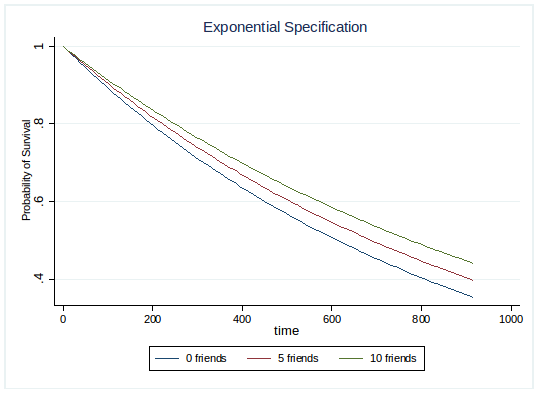
\includegraphics[scale=0.65]{exponential.png}
\end{figure}

The file ``survival.dta'' contains the predicted survival probability for individuals with 0, 5 and 10 friends (evaluated at means for the other covariates). The statement did not specify a point in time, but we find a coincidence with the statement at $t=330.76$ (average days of imprisonment was $131.62$). 

\paragraph{Table 3 with regiment fixed effects}
page 1476, line 2. ``Even when we included state of regiment fixed effects, the hazard ratio on the number of friends remained virtually unchanged (e.g. the hazard ratio on the initial number of friends was $0.976$, $=0.009$).''

\begin{sidewaystable}
\caption{Table 3 with regiment state effects}\footnote{Company clustered standard errors are in parentheses. Symbols ++, +, and * indicate statistical significance levels of 1, 5, and 10 percent respectively.}
\begin{tabular}{lllllll}
\hline
                                         & Hazard rate & Std. err & Hazard rate & Std. err & Hazard rate & Std. err \\
Number of friends                        & 0.984*      & -0.009   & 0.978       & -0.009   &             &          \\
Initial number of friends                &             &          &             &          & 0.976++     & -0.009   \\
Ln(number of prisoners in camp)          &             &          & 1.538++     & -0.141   & 1.525++     & -0.14    \\
Fraction of company dying before capture & 1.427       & -1.227   & 1.19        & -1.011   & 0.787       & -0.653   \\
Professional or proprietor               & 0.512       & -0.134   & 0.506++     & -0.131   & 0.502++     & -0.13    \\
Artisan                                  & 0.862       & -0.114   & 0.862       & -0.114   & 0.851       & -0.112   \\
Laborer                                  & 1.163       & -0.148   & 1.154       & -0.146   & 1.141       & -0.145   \\
German                                   & 1.135       & -0.213   & 1.116       & -0.21    & 1.103       & -0.206   \\
Irish                                    & 0.731*      & -0.118   & 0.723       & -0.116   & 0.723       & -0.115   \\
British                                  & 0.616*      & -0.167   & 0.630*      & -0.17    & 0.637*      & -0.174   \\
Other                                    & 0.612       & -0.145   & 0.603       & -0.144   & 0.602       & -0.143   \\
Sergeant, corporal or officer            & 0.570++     & -0.117   & 0.561++     & -0.113   & 0.557++     & -0.112   \\
Age at captivity                         & 1.042++     & -0.008   & 1.040++     & -0.007   & 1.040++     & -0.007   \\
Height at enlistment                     & 1.014*      & -0.007   & 1.014*      & -0.007   & 1.014*      & -0.007   \\
Observations                             & 3026        &          & 3026        &          & 3026        &          \\
Number of subjects                       & 23174       &          & 23174       &          & 23174       &          \\
Log pseudo likelihood                    & -1307.77    &          & -1291.45    &          & -1290.674   &          \\
\end{tabular}
\end{sidewaystable}

\paragraph{Table 3 with splines}
page 1476, line 6 and footnote 23 ``Our experiments with splines suggested that the marginal effect of a friend on survival was greater for the first two friends than for more."  Footnote 23: "The hazard rate on the marginal effect of fewer than three friends was $0.956$ ($=0.044$) and the hazard rate on the marginal effect of three or more friends was $0.980$ ($=0.011$). Although the first hazard rate was not statistically significantly different from one, the two terms together were jointly significant.''

\begin{table}[ht]
\centering
\caption{Spline at 3}
\begin{tabular}{ll}
\hline
                     & Hazard rate \\
Fewer than 3 friends & 0.956       \\
                     & -0.0443     \\
3 or more friends    & 0.980*      \\
                     & -0.0108     \\
Observations         & 23256       \\
Chi-sq               & 7.789       \\
Prob > chi-sq        & 0.0204      \\
\end{tabular}
\end{table}

\paragraph{Weibull specification}
page 1477, line 12. ``When we use a Weibull rather than an exponential specification, we found no evidence of duration dependence...''

\begin{sidewaystable}
\caption{Weibul}\footnote{Company clustered standard errors are in parentheses. Symbols ++, +, and * indicate statistical significance levels of 1, 5, and 10 percent respectively.}
\begin{tabular}{llllllllll}
\hline
                                         & \multicolumn{2}{l}{Specification 1} & \multicolumn{2}{l}{Specification 2} & \multicolumn{2}{l}{Specification 3} \\
VARIABLES                                & Hazard rate                         & Std. err.                           & Hazard rate                         & Std. err. & Hazard rate & Std. err. \\
Number of friends                        & 0.986                               & -0.009                              & 0.979                               & -0.009 &  &  \\
Initial number of friends                &                                     &                                     &                                     &  & 0.977++ & -0.009 \\
Ln(number of prisoners in camp)          &                                     &                                     & 1.531++                             & -0.139 & 1.517++ & -0.139 \\
Fraction of company dying before capture & 1.242                               & -0.897                              & 1.008                               & -0.722 & 0.733 & -0.525 \\
Professional or propietor                & 0.566                               & -0.147                              & 0.562                               & -0.144 & 0.554 & -0.142 \\
Artisan                                  & 0.95                                & -0.121                              & 0.952                               & -0.12 & 0.942 & -0.119 \\
Laborer                                  & 1.308                               & -0.157                              & 1.303                               & -0.154 & 1.296 & -0.154 \\
German                                   & 1.198                               & -0.218                              & 1.169                               & -0.212 & 1.153 & -0.209 \\
Irish                                    & 0.771                               & -0.123                              & 0.765*                              & -0.12 & 0.753* & -0.118 \\
British                                  & 0.630*                              & -0.17                               & 0.644                               & -0.174 & 0.646 & -0.176 \\
Other                                    & 0.656*                              & -0.155                              & 0.643*                              & -0.153 & 0.640* & -0.151 \\
Sargeant, corporal or officer            & 0.536++                             & -0.114                              & 0.531++                             & -0.11 & 0.528++ & -0.11 \\
Age at captivity                         & 1.046++                             & -0.008                              & 1.045++                             & -0.008 & 1.045++ & -0.008 \\
Height at entlistment                    & 1.01                                & -0.007                              & 1.01                                & -0.007 & 1.011 & -0.007 \\
Observations                             & 23256                               &                                     & 23256                               &  & 23256 &  \\
Log pseudo likelihood                    & -1322.852                           &                                     & -1306.836                           &  & -1305.627 &  \\
Duration dependence                      & 1.088                               &                                     & 1.08                                &  & 1.084 &  \\
\end{tabular}
\end{sidewaystable}

\paragraph{Month dummies}
page 1477, line 19. ``When we included dummy variables in our specification indicating that an individual had survived 1, 2, 3 or more months, we found that those who had survived one or two months were less likely to die than those still in their first month of captivity, but that the advantage of having survived a third month was small and there was no advantage to having survived a fourth month.''

\begin{sidewaystable}
\caption{controlling for months survived}\footnote{Company clustered standard errors are in parentheses. Symbols ++, +, and * indicate statistical significance levels of 1, 5, and 10 percent respectively.}
\begin{tabular}{lllllll}
\hline
                                         & \multicolumn{2}{l}{Specification 1} & \multicolumn{2}{l}{Specification 2} & \multicolumn{2}{l}{Specification 3} \\
                                         & Hazard rate                         & Std. err.                           & Hazard rate                         & Std. err. & Hazard rate & Std. err. \\
Number of friends                        & 0.989                               & -0.009                              & 0.982*                              & -0.009 &  &  \\
Initial number of friends                &                                     &                                     &                                     &  & 0.977++ & -0.009 \\
Ln(number of prisoners in camp)          &                                     &                                     & 1.612++                             & -0.146 & 1.604++ & -0.145 \\
Fraction of company dying before capture & 1.368                               & -1.001                              & 1.117                               & -0.811 & 0.832 & -0.603 \\
Professional or propietor                & 0.56                                & -0.145                              & 0.557                               & -0.142 & 0.547 & -0.14 \\
Artisan                                  & 0.946                               & -0.121                              & 0.951                               & -0.121 & 0.939 & -0.12 \\
Laborer                                  & 1.302                               & -0.158                              & 1.302                               & -0.156 & 1.298 & -0.156 \\
German                                   & 1.22                                & -0.223                              & 1.195                               & -0.216 & 1.178 & -0.213 \\
Irish                                    & 0.774                               & -0.125                              & 0.770*                              & -0.122 & 0.756* & -0.12 \\
British                                  & 0.618*                              & -0.168                              & 0.632*                              & -0.172 & 0.634* & -0.174 \\
Other                                    & 0.658*                              & -0.156                              & 0.650*                              & -0.156 & 0.647* & -0.154 \\
Sargeant, corporal or officer            & 0.533++                             & -0.114                              & 0.531++                             & -0.111 & 0.526++ & -0.11 \\
Age at captivity                         & 1.047++                             & -0.008                              & 1.046++                             & -0.008 & 1.045++ & -0.008 \\
Height at entlistment                    & 1.01                                & -0.007                              & 1.01                                & -0.007 & 1.011 & -0.007 \\
Survived 1 month                         & 0.407++                             & -0.08                               & 0.362++                             & -0.072 & 0.352++ & -0.071 \\
Survived 2 months                        & 0.472++                             & -0.092                              & 0.401++                             & -0.08 & 0.393++ & -0.078 \\
Survived 3 months                        & 0.74                                & -0.137                              & 0.64                                & -0.12 & 0.631 & -0.118 \\
Survived 4 or more months                & 0.833                               & -0.134                              & 0.745*                              & -0.12 & 0.740* & -0.119 \\
Observations                             & 23256                               &                                     & 23256                               &  & 23256 &  \\
Log pseudo likelihood                    & -1307.333                           &                                     & -1287.9                             &  & -1285.595 &  \\
\end{tabular}
\end{sidewaystable}

\paragraph{Cox Proportional Hazard Model}
page 1477, line 26 footnote.
``We also investigated the use of a Cox proportional hazard model to allow the baseline hazard to rise or fall in any month. Controlling for camp conditions, we obtained a statistically insignificant hazard ratio on friends of $0.987$ ($=0.009$). We suspect that we are losing power because of our small sample size.''

\begin{sidewaystable}
\caption{Cox proportional models}\footnote{Company clustered standard errors are in parentheses. Symbols ++, +, and * indicate statistical significance levels of 1, 5, and 10 percent respectively.}
\begin{tabular}{lllllll}
\hline
                                         & Hazard rate & Std. err. & Hazard rate & Std. err. & Hazard rate & Std. err. \\
Number of friends                        & 0.992       & -0.009    & 0.987       & -0.009    &             &           \\
Initial number of friends                &             &           &             &           & 0.978       & -0.009    \\
Ln(number of prisoners in camp)          &             &           & 1.593++     & -0.149    & 1.587++     & -0.149    \\
Fraction of company dying before capture & 1.751       & -1.298    & 1.558       & -1.148    & 1.179       & -0.867    \\
Professional or propietor                & 0.557       & -0.144    & 0.556       & -0.142    & 0.546       & -0.139    \\
Artisan                                  & 0.942       & -0.121    & 0.952       & -0.122    & 0.938       & -0.12     \\
Laborer                                  & 1.284       & -0.157    & 1.287       & -0.157    & 1.284       & -0.156    \\
German                                   & 1.241       & -0.228    & 1.218       & -0.223    & 1.2         & -0.22     \\
Irish                                    & 0.765       & -0.126    & 0.763*      & -0.123    & 0.746*      & -0.121    \\
British                                  & 0.613*      & -0.166    & 0.625*      & -0.169    & 0.626*      & -0.171    \\
Other                                    & 0.658*      & -0.159    & 0.652*      & -0.159    & 0.649*      & -0.158    \\
Sargeant, corporal or officer            & 0.538++     & -0.115    & 0.537++     & -0.113    & 0.532++     & -0.112    \\
Age at captivity                         & 1.048++     & -0.008    & 1.046++     & -0.008    & 1.046++     & -0.008    \\
Height at entlistment                    & 1.01        & -0.008    & 1.01        & -0.007    & 1.011       & -0.007    \\
Observations                             & 23256       &           & 23256       &           & 23256       &           \\
Log pseudo likelihood                    & -3102.845   &           & -3086.134   &           & -3083.63    &           \\
\end{tabular}
\end{sidewaystable}

\begin{table}[ht]
\centering
\caption{table 4 net transfer}\footnote{Company clustered standard errors are in parentheses. Symbols ++, +, and * indicate statistical significance levels of 1, 5, and 10 percent respectively.}
\begin{tabular}{lll}
\hline
VARIABLES               & Hazard Rate & Std. err. \\
Net transfer of friends & 0.946**     & -0.024    \\
Observations            & 15998       &           \\
\end{tabular}
\end{table}

\paragraph{On limiting the sample}
page 1480, line 17. ``When we restricted the sample to exclude deaths after September 1864 and captures prior to October 1864 because only the dying may have been left at Andersonville once men were transferred out, our results remained unchanged. The derivative of the coefficient on the number of men in the company was 0.003 (sdev=0.001) and the derivative of the coefficient on the number of men in the regiment with the same last name was 0.035 (sdev=0.007).''

\paragraph{On the mortality of privates}
page 1480, line 54. ``The fraction of sergeants or higher rank is not a reflection of own officer mortality. When we restricted the sample to privates, we found that the derivative of this coefficient was 0.115 (sdev=0.054).''

\paragraph{On the role of networks in predicting escape from Andersonville}
page 1482, line 25. ``Also suggestive of friends not always helping survival is that, among the men at Andersonville, we find no evidence that the number of friends predicted whether an individual was one of the 140 escaped.''

See table below for the final three verifications:

\begin{sidewaystable}
\caption{Final three specifications}\footnote{Company clustered standard errors are in parentheses. Symbols ++, +, and * indicate statistical significance levels of 1, 5, and 10 percent respectively.}
\begin{tabular}{llll}
\hline
                                                 & Dependent variable: Lived & Dependent variable: Lived & Dependent variable: Escaped \\
                                                 & Shorter time period       & Privates only             &                             \\
Number of men in company                         & 0.003++                   & 0.003++                   & 0                           \\
                                                 & -0.001                    & -0.001                    & 0                           \\
Fraction of company with rank sergeant or higher & 0.115                     & 0.139++                   & -0.001                      \\
                                                 & -0.054                    & -0.036                    & -0.002                      \\
Number of men with same last name in regiment    & 0.033++                   & 0.035++                   & 0                           \\
                                                 & -0.007                    & -0.007                    & 0                           \\
Log(number of men in camp from same town)        & -0.003                    & -0.001                    & 0                           \\
                                                 & -0.005                    & -0.005                    & 0                           \\
Pseudo R2                                        & 0.036                     & 0.047                     & 0.015                       \\
Observations                                     & 25880                     & 27923                     & 28190                       \\
\end{tabular}
\end{sidewaystable}

The only in-text claim that we are not able to confirm is their statement that there is no mortality difference between the colored non-officers and the rest of the Andersonville POWs (page 1480, footnote 29) as we don’t have any information on the race of the POWs.

\section*{Appendix: Non-parametric estimation}
The following figures are our replications of the Kaplan-Meier survival estimates which show no differences to the original:

\begin{figure}
\centering
\caption{Kaplan-Meier survival estimate}
\label{kmSurvival}
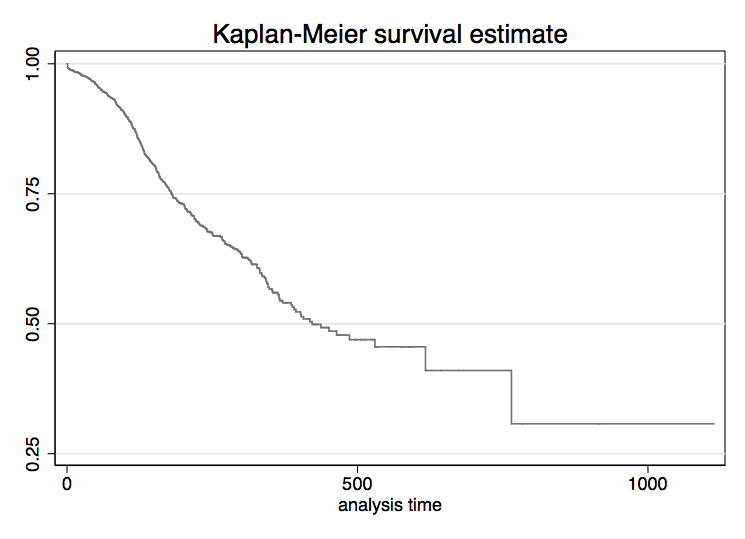
\includegraphics[scale=0.3]{kaplan1.png}
\end{figure}

\begin{figure}
\centering
\caption{Kaplan-Meier survival estimates by early and late capture date}
\label{kmCapture}
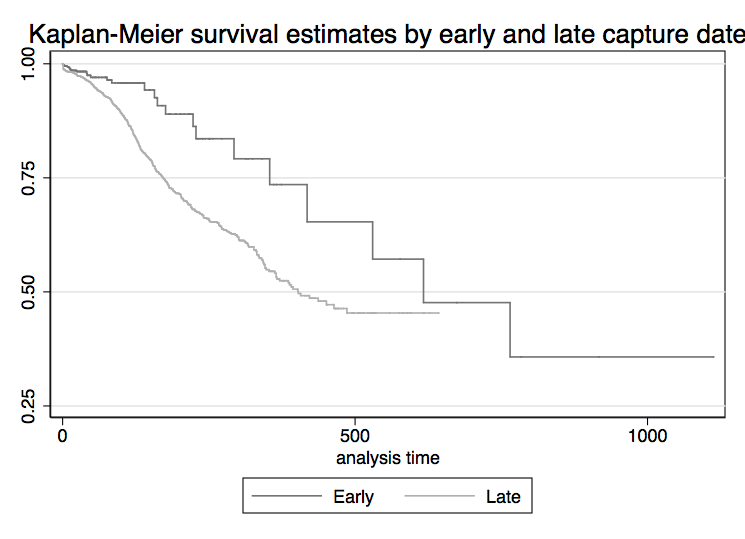
\includegraphics[scale=0.3]{kaplan2.png}
\end{figure}

\begin{figure}
\centering
\caption{Kaplan-Meier survival estimates by camp for late captures}
\label{kmCamp}
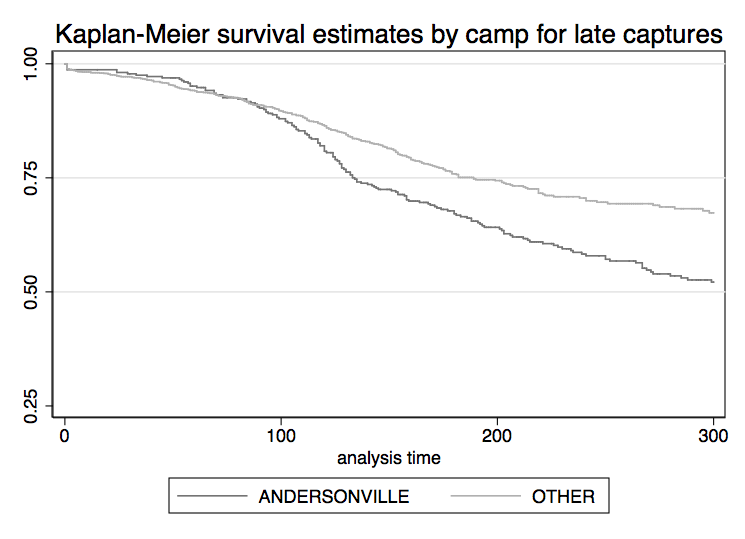
\includegraphics[scale=0.3]{kaplan3.png}
\end{figure}

\begin{figure}
\centering
\caption{Kaplan-Meier survival estimates by number of friends for Anderson}
\label{kmNumber}
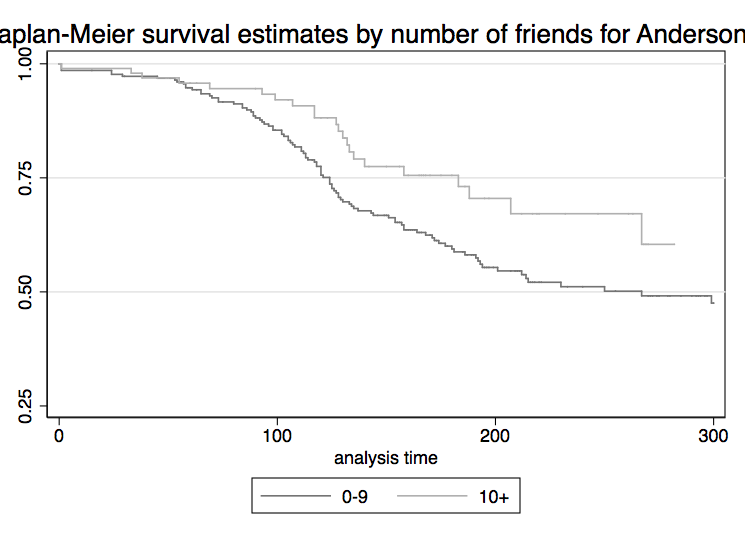
\includegraphics[scale=0.3]{kaplan4.png}
\end{figure}

\printbibliography

\end{refsection}